
\documentclass[runningheads]{llncs}

\usepackage{graphicx}
\usepackage{amsmath,amssymb,amsfonts}
\usepackage{algorithmic}
\usepackage{graphicx}
\usepackage{textcomp}
\usepackage{amsmath}
\usepackage{listings}%
\usepackage{graphicx}%
\usepackage{multirow}%
\usepackage{amsmath,amssymb,amsfonts}%
\usepackage{amsthm}%
\usepackage{mathrsfs}%
\usepackage[title]{appendix}%
\usepackage{xcolor}%
\usepackage{textcomp}%
\usepackage{manyfoot}%
\usepackage{booktabs}%
\usepackage{algorithm}%
\usepackage{algorithmicx}%
\usepackage{algpseudocode}%
\usepackage{listings}%


\begin{document}

\title{Preserving Integrity of Electronic Health Record (EHR) in Multi-Cloud Environment}

\author{Uday Yadav\orcidID{0009-0006-4188-5097} \and
Dr. Narendra V G\orcidID{0000-0002-6259-0056}}

\authorrunning{}

\institute{Department of Computer Science and Engineering, Manipal Institute of Technology, Manipal Academy of Higher Education, Manipal- 576 104, Karnataka, India
\email{yadav117uday@gmail.com}\\
\email{narendra.vg@manipal.edu}
}

%
\maketitle             
%

\vspace{-0.5cm}

\begin{abstract}
Electronic Health Records (EHR) are sensitive documents that require a secure storage environment. Various research and regulatory standards have established a security framework to protect such documents in the cloud from malicious access and manipulation. But as cloud usage expands to multi-cloud environments, a new set of challenges arises, like integrity and data in-consistency of documents in the system. This research aims to preserve the integrity of EHR documents in a multi-cloud environment. 

\keywords{EHR \and Multi-Cloud \and Data Integrity}
\end{abstract}

\vspace{-0.5cm}

\section{Introduction}

The Government of India's flagship initiative, the Digital India Movement, aims to empower India through National Health Portal which offers details on illnesses and ailments, medical professionals, and therapies and the Ayushman Bharat Digital Mission seeks to establish a digital health ID for each Indian citizen with a platform that enables patients to access their medical records from any location in the nation. 

Digitization of electronic medical records requires infrastructure that is secure, reliable and scalable such that it can fulfill the compute capacity to serve the demand of millions of individuals. Cloud storage for electronic medical records in India offers numerous advantages such as scalability, allowing healthcare organizations to expand their storage needs as data grows. It offers robust security features, protecting patient data from breaches and unauthorized access and enhanced data accessibility, making them a cost-effective choice, especially for resource-constrained healthcare settings in India. 

Multi-cloud offers the advantage of diversification, reducing vendor lock-in risk and providing flexibility to choose the best services and pricing from multiple cloud providers. In a multi-cloud setup, the risk of data integrity issues related to malicious manipulation is amplified, as attackers may exploit vulnerabilities across different cloud providers to tamper with or corrupt data, necessitating stringent security measures and monitoring to safeguard against such threats. 

The likelihood of a breach of patient privacy and confidentiality increases when electronic health records, or EHRs, are used and exchanged between various healthcare providers. Since sensitive information about the patient is contained in the medical records, a violation of privacy and confidentiality exposes the patient and caregivers to stress, discrimination, and defamation.  Because electronic health records are more likely to be altered or destroyed by unauthorized individuals, maintaining their integrity is crucial. The necessity for sophisticated security protection mechanisms has arisen because of the sensitive nature of the data found in Electronic Health Records. 

\section{Related Work}

Raghavendra Ganiga et al [1] address security concerns for storing healthcare data in the cloud by proposing a framework offering multiple solutions. Highlighted methods include access control and data storage lock algorithms, emphasizing the importance of robust security for cloud-based EHR systems.

P. Vimalachandran et al [2] tackle the critical issue of data integrity in EHRs by proposing a comprehensive framework that goes beyond mere data accuracy, encompasses robust information governance, effective patient identification, authorship validation, and tamper-proof record-keeping, highlighting the multifaceted nature of data integrity and its crucial role in ensuring trustworthy and reliable EHR. 

Vidya and K. Vani et al [3] propose a revolutionary method for securing Personal Health Records (PHRs) in the cloud using homomorphic encryption and data auditing. This patient-centric approach grants individuals control over their privacy by encrypting PHRs on cloud servers while enabling authorized access and verification without decryption, safeguarding sensitive health information in the digital healthcare landscape.  

Zongda Wu [4] research focuses on securing electronic medical records (EHRs) in the cloud, introducing hierarchical storage and segmentation query models. These aim to boost EHR security in untrusted cloud environments without sacrificing data availability, emphasizing the crucial balance between security and accessibility in handling sensitive medical information.

Umar Abdulkadir et al [5] research introduces the "Ring Learning with Error (RLWE)" encryption scheme as a solution to overcome various challenges in EHR management. The existing problems include slow processing speed, weak security mechanisms, high computational overheads, and vulnerabilities in public-private key pairs.

Wenxin Hu et al [7] present a lattice-based ring signature scheme specifically designed for secure cloud-based EHR sharing. This scheme offers several key benefits, including correctness, anonymity, and unforgeability. It claims to outperform other existing schemes, emphasizing the importance of user anonymity and the unforgeability of electronic medical records and their associated signatures. 

Léonore Cellier et al [9] addresses cybersecurity in the e-health sector, outlining key success factors. It conducts an in-depth analysis of the current EHR system in Swiss hospitals, and further proposes strategies to enhance EHR security and trust, including GDPR compliance, implementing organizational controls, revising legal frameworks for staff, and empowering patients to manage their records through technological measures. 

Deepali Awasthi et al [14] delves into cutting-edge privacy-preserving techniques for EHRs within cloud computing and blockchain environments, encompassing methods such as zero-knowledge proofs, attribute-based encryption, and quasi-identifier recognition. 
\section{Methodology}

\subsection{Establishing integrity of EHR}

To establish integrity of EHR documents, we first need to establish authenticity, non-repudiation and integrity for the document. This ensures that what we are protecting is unerringly the correct information, can be achieved through using various digital signature cryptographic schemes.

\begin{enumerate} 

    \item  \textbf{Step 1 : Calculate SHA Hash of the document} \\ 
    Calculating the Secure Hash Algorithm (ex SHA-512) of the document is crucial for secure storage as it ensures data integrity and pre-image resistance. Any minor change in the document results in a drastically different hash, allowing verification of the document’s integrity.
    \item \textbf{Step 2 : Digital Signatures for documents} \\ 
    Set up a digital signature infrastructure that includes both public and private keys. Digital signatures are crucial for ensuring the authenticity and integrity of EHR documents. They confirm that the document has not been tampered with and that it was indeed created by the authorized practitioner.
    \item \textbf{Step 3 : Setup event logging system} \\ 
    Event logging systems establish non-repudiation by securely recording all activities, creating an indisputable record tied to a user or event. This prevents users from denying their actions. The system ensures the logs have not been tampered with, typically using cryptographic techniques like digital signatures and hash functions. This provides a robust mechanism for accountability and traceability.
\end{enumerate}

\vspace{-0.5cm}

\begin{figure}
\centerline{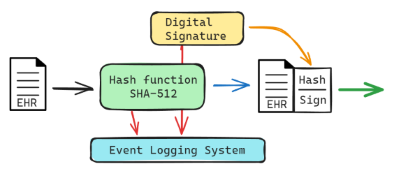
\includegraphics{img/step1.png}}
\caption{Establishing integrity of EHR}
\label{fig}
\end{figure}

\subsection{Ensuring consistency and security in distributed storage}

In a multi-cloud environment for Electronic Health Records (EHR) storage, ensuring data consistency is paramount for maintaining the integrity and reliability of healthcare information. Achieving data consistency involves implementing robust synchronization mechanisms across multiple cloud providers to ensure that updates and modifications to EHR data are uniformly applied and reflected in real-time across all cloud instances. 

Lightweight synchronization mechanism based on a simple text-log is proposed for implementation, ensuring the successful saving of Electronic Medical Records (EHR) documents across multiple cloud storage environments. The mechanism involves the creation of a distributed log (full replication mode) that records all transactions related to EHR document storage and updates. Each cloud instance maintains a local copy of this log, and any modification to an EHR document triggers a log entry. Periodically, cloud instances exchange log entries and reconcile differences to synchronize their states. This approach is lightweight as it leverages a simplified log structure and minimizes the need for continuous real-time synchronization, reducing the impact on performance. Additionally, the use of checksums or hash functions within the log entries can enhance data integrity verification during synchronization. 

\vspace{-0.5cm}

\begin{figure}
\centerline{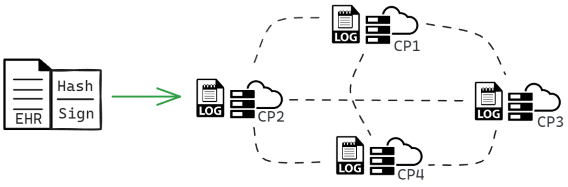
\includegraphics{img/step2.png}}
\caption{Establishing integrity of EHR}
\label{fig}
\end{figure}

\vspace{-0.5cm}

By adopting this lightweight log-based mechanism, healthcare systems can achieve reliable and consistent EHR document storage across multi-cloud environments while minimizing the computational overhead should have the following feature set : 


\begin{enumerate}    
\item \textbf{Log Creation and Structure} 
A distributed log is the synced across all storage system is established to record transactions related to EHR document storage. This log is designed to be simple, containing essential information such as document ID, timestamp, type of operation (create, update, delete), and any additional metadata required for synchronization.

\item \textbf{Local Log Maintenance} Each cloud instance maintains a local copy of the log, tracking all modifications to EHR documents within its jurisdiction. Any change triggers the creation of a log entry, providing a comprehensive history of document transactions.

\item \textbf{Asynchronous Log Verfication} Periodically, cloud instances asynchronously exchange their log entries with one another. This exchange can be scheduled at predefined intervals or triggered by significant events, such as the completion of a critical operation.

\item \textbf{Reconciliation and Synchronization} During log exchange, cloud instances compare and reconcile their logs. Differences in log entries indicate variations in document states. The synchronization process ensures that each instance updates its local copy of the EHR document based on the reconciled log entries.

\item \textbf{Data Integrity Verification} To enhance data integrity, checksums or hash functions can be incorporated into the log entries. This allows each cloud instance to verify the integrity of received log entries, minimizing the risk of data corruption during synchronization.

\item \textbf{Conflict Resolution} In the event of conflicting log entries (e.g., simultaneous updates to the same document from different instances), a conflict resolution mechanism is employed. This may involve prioritizing the entry with the latest timestamp or implementing predefined rules for conflict resolution.

\end{enumerate}

This verification mechanism enables patients and third-party users to access and verify the integrity of EHR documents stored using the proposed lightweight synchronization mechanism in a easy and convenient way. 

\section{Result \& Analysis}

We conducted a abbreviated evaluation of the proposed lightweight synchronization mechanism for preserving the integrity of Electronic Health Records (EMR) in a multi-cloud environment.

\begin{table}[]
\centering
\caption{Analysis Based on Various Threat scenarios }
\label{tab:my-table}
\begin{tabular}{|l|l|l|l|}
\hline
Susceptibility &
  Description &
  Impact &
  Mitigation \\ \hline
Data Consistency &
  \begin{tabular}[c]{@{}l@{}}Possibility of inconsistency \\ due to network delays or \\ conflicts simultaneous \\ updates from 
 instances\end{tabular} &
  \begin{tabular}[c]{@{}l@{}}Risk of outdated or \\ conflicting data across \\ instances, \\ compromising integrity \end{tabular} &
  \begin{tabular}[c]{@{}l@{}}Cross checking the \\ timestamp from log \\ verifies the version \\ of document \end{tabular} \\ \hline
\begin{tabular}[c]{@{}l@{}}Synchronization \\ Efficiency\end{tabular} &
  \begin{tabular}[c]{@{}l@{}}Potential delays or resource \\ bottlenecks during the \\ synchronization process\end{tabular} &
  \begin{tabular}[c]{@{}l@{}}Degraded system \\ performance, leading \\ to slower updates\end{tabular} &
  \begin{tabular}[c]{@{}l@{}}Performing asynchro \\ -nous log sychroni \\ -zation decreases time.\end{tabular} \\ \hline
\begin{tabular}[c]{@{}l@{}}Cryptographic \\ Verification\end{tabular} &
  \begin{tabular}[c]{@{}l@{}}Vulnerability in the PKI \\ components leading to \\ unauthorized access or \\ compromised signatures\end{tabular} &
  \begin{tabular}[c]{@{}l@{}}Risk of tampering \\ of sensitive \\ healthcare data\end{tabular} &  \begin{tabular}[c]{@{}l@{}}Protect private keys \\ by employing strong \\ encryption algorithms \end{tabular} \\ \hline
Access Control &
  \begin{tabular}[c]{@{}l@{}}Inadequate access controls \\ may result in unauthorized \\ parties gaining access to \\ EMR documents\end{tabular} &
  \begin{tabular}[c]{@{}l@{}}Unauthorized access \\ to sensitive medical \\ information\end{tabular} &
  \begin{tabular}[c]{@{}l@{}}Use LDAP or \\ Azure AD and \\  monitor access \\ usage by users\end{tabular} \\ \hline

\end{tabular}
\end{table}

\section{Conclusion}

The paper introduces a design framework for preserving the integrity of Electronic Medical Records (EHR) in a Multi-Cloud Environment, addressing the critical challenges of data consistency and security. A lightweight synchronization mechanism, relying on a simple log structure, ensures uniform updates across multiple cloud instances while minimizing computational overhead. This mechanism incorporates cryptographic techniques, transaction management through log-based system and digital signatures. Patients and third-party users can independently verify the integrity of EHR documents through a secure and user-friendly interface, enhancing transparency and trust. The paper emphasizes the importance of data integrity in healthcare information exchange, presenting a holistic solution that combines synchronization efficiency with robust cryptographic verification, ultimately contributing to the reliability and security of EHR storage in multi-cloud environments.

\begin{thebibliography}{00}

\bibitem{b1} T. Piliouras, P. Tague, and A. A. Ghorbani, "Trust in a cloud-based healthcare environment," 2011 8th International Conference \& Expo on Emerging Technologies for a Smarter World, Hauppauge, NY, USA, 2011, pp. 1-6, doi: 10.1109/CEWIT.2011.6135890.

\bibitem{b2} Ganiga, Raghavendra and Pai, Radhika and M M, Manohara and Sinha, Rajesh. (2020). Security framework for cloud-based electronic health record (EHR) system. \textit{International Journal of Electrical and Computer Engineering (IJECE)}, 10(1), 455-466. DOI: 10.11591/ijece.v10i1.pp455-466.

\bibitem{b3} P. Vimalachandran, H. Wang, Y. Zhang, B. Heyward and F. Whittaker, "Ensuring data integrity in electronic health records: A quality health care implication," 2016 International Conference on Orange Technologies (ICOT), Melbourne, VIC, Australia, 2016, pp. 20-27, doi: 10.1109/ICOT.2016.8278970.

\bibitem{b4} Wu, Zongda \& Xuan, Shaolong \& Xie, Jian \& Lin, Chongze \& Lu, Chenglang. (2022). How to ensure the confidentiality of electronic medical records on the cloud: A technical perspective. Computers in Biology and Medicine. 147. 105726. 10.1016/j.compbiomed.2022.105726. 

\bibitem{b5} U. Abdulkadir, V. O. Waziri, J. K. Alhassan and I. Ismaila, "Ring Learning With Error-Based Encryption Scheme for the Privacy of Electronic Health Records Management," 2022 5th Information Technology for Education and Development (ITED), Abuja, Nigeria, 2022, pp. 1-5, doi: 10.1109/ITED56637.2022.10051260

\bibitem{b6} Chang Xu, Zijian Chan, Liehuang Zhu, Rongxing Lu, Yunguo Guan, Kashif Sharif, Efficient and privacy-preserving similar electronic medical records query for large-scale ehealthcare systems, Computer Standards \& Interfaces, Volume 87, 2024, 103746, ISSN 0920-5489, https://doi.org/10.1016/j.csi.2023.103746.

\bibitem{b7} W. Hu, Y. Chai, X. Chen and C. Zheng, "Lattice based Ring Signature Scheme for Secure Cloud-based EMR Sharing," 2022 7th International Conference on Computer and Communication Systems (ICCCS), Wuhan, China, 2022, pp. 789-794, doi: 10.1109/ICCCS55155.2022.9845850.

\bibitem{b8} S. S. Vellela, B. Venkateswara Reddy, K. K. Chaitanya and M. V. Rao, "An Integrated Approach to Improve E-Healthcare System using Dynamic Cloud Computing Platform," 2023 5th International Conference on Smart Systems and Inventive Technology (ICSSIT), Tirunelveli, India, 2023, pp. 776-782, doi: 10.1109/ICSSIT55814.2023.10060945.

\bibitem{b9} Cellier, Leonore and Ghernaouti, Solange. (2019). {An interdisciplinary approach for security, privacy and trust in the electronic medical record: A pragmatic legal perspective}, 1-6. DOI: 10.1109/HealthCom46333.2019.9009588.

\bibitem{b10} A. P. Vinnarasi, R. Dayana, P. Malarvezhi and K. Vadivukkarasi, "E-Health Security on Cloud Computing and its Challenges," 2022 First International Conference on Artificial Intelligence Trends and Pattern Recognition (ICAITPR), Hyderabad, India, 2022, pp. 1-9, doi: 10.1109/ICAITPR51569.2022.9844196.

\bibitem{b11} Xinglong Zhang, Peng Xi, Wenjuan Liu, and Shaoliang Peng. 2023. EMRShareChain: A Privacy-Preserving EMR Sharing System Model Based on the Consortium Blockchain. In Bioinformatics Research and Applications: 18th International Symposium, ISBRA 2022, Haifa, Israel, November 14–17, 2022, Proceedings. Springer-Verlag, Berlin, Heidelberg, 343–355.

\bibitem{b12} Wishah, Raed \& Alali, Haitham. (2017). Health Information Privacy and Security Framework: Supporting Electronic Medical Records in Healthcare Systems. International Journal of Business Innovation and Research. 8.

\bibitem{b13} Savitz, Samuel \& Savitz, Lucy \& Fleming, Neil \& Shah, Nilay \& Go, Alan. (2020). How much can we trust electronic health record data?. Healthcare. 8. 100444. 10.1016/j.hjdsi.2020.100444.

\bibitem{b14} Deepali Awasthi, Shagun Chauhan, Dr. Hitesh Singh, Swati Lohiya, Mahima Kaushik, Dr. Vivek Kumar, 2023, Safeguarding the Confidentiality of Electronic Health Records:, INTERNATIONAL JOURNAL OF ENGINEERING RESEARCH \& TECHNOLOGY (IJERT) Volume 12, Issue 05 (May 2023).

\bibitem{b15} Vani.K, Vidya.S,. 2013. “Secured PHR Transactions Using Homomorphic Encryption in Cloud Computing”. International Journal of Engineering and Computer Science 2 (12).

\end{thebibliography}

\end{document}
